%% ch04-nisq-optimization.tex — Chapter V (RQ2): Hardware-Aware Optimization on Noisy Devices (DEAL and QAWA)
%% STE-edited version (ASD-STE100 style, ~80% strictness) of chapters/ch04-nisq-optimization.tex
\chapter{Hardware-Aware Optimization on Noisy Devices}\label{ch:nisq}

This chapter addresses RQ3: how optimisation algorithms on noisy intermediate-scale quantum (NISQ) devices can use the structure of the problem and of the hardware instead of black-box search over circuit parameters. The quantum approximate optimisation algorithm (QAOA) and its variational relatives promise to solve combinatorial problems on today's processors. In practice, their classical outer loop consumes thousands of noisy circuit evaluations. Their landscapes flatten as circuits deepen, and their output distributions are hard to interpret and impossible to verify at scale. We present two responses.

Part~A introduces \deal, Direct Entanglement Ansatz Learning. \deal\ derives the circuit angles directly from the coefficients of the quadratic unconstrained binary optimisation (QUBO) problem. It places the logical qubits on the physical device according to the same coefficients and the device's calibration data. It entangles them with a mixer of maximally entangling native gates, and it mitigates the residual noise with an adaptive digital zero-noise extrapolation. Part~B introduces \qawa, the Quantum Approximate Walk Algorithm. \qawa\ replaces the problem-derived ansatz by a \emph{classical-data-traceable} oracle of linear two-qubit depth. It learns approximate solution patterns through a distributed quantum-walk procedure, and it makes the outputs interpretable and verifiable in polynomial time through classical preprocessing of mid-circuit measurement data.

Both methods were validated on IBM Heron processors, and both were first checked with the GPU simulation pipeline of \cref{ch:qgear}. The chapter closes with a contrast of the two sources of structure, the problem and the data, and shows how the second leads into the vectorised encodings of \cref{ch:qml}.

\section{Introduction and Motivation}\label{sec:nisq:intro}

Combinatorial optimisation is the application most often proposed for near-term quantum computers, and QAOA \cite{farhi2014qaoa} is the algorithm most often proposed for it. The reasons are practical. QAOA circuits are shallow, and their structure follows directly from the cost function. Any problem that can be written as a QUBO can be run without further algorithmic invention. Such problems include MaxCut, the travelling salesman problem (TSP), knapsack, portfolio selection and many others \cite{glover2018qubo}.

The difficulties are equally practical and documented extensively \cite{abbas2024challengesqopt,weidenfeller2022qaoascaling,cerezo2021vqa}. QAOA is a variational algorithm. For a circuit of $p$ layers, a classical optimiser must find the $2p$ angles $(\bm{\gamma},\bm{\beta})$. The optimiser treats the quantum processor as a black box and evaluates the energy at hundreds or thousands of parameter settings. Each evaluation costs thousands of shots on a device whose calibration drifts over the hours that such a run takes. Shot noise and gate errors corrupt the landscape that the optimiser sees.

As the number of qubits and layers grows, the landscape becomes exponentially flat \cite{mcclean2018barren}, and the optimiser converges to spurious minima or not at all. Deeper circuits should approximate the optimum better. But on hardware, each additional layer adds two-qubit gates whose errors compound. Beyond a device-dependent depth, the output distribution collapses toward uniform noise. Finally, even when the algorithm returns a good bit string, it is hard to say \emph{why}. The output is a sample from an entangled state, which cannot be reconstructed without state tomography, whose cost grows exponentially with the number of qubits.

The thesis statement of this dissertation (\cref{ch:intro}) proposes co-design as the remedy: the algorithm should use the structure available to it rather than rediscover it by search. In the optimisation setting, two sources of structure exist, and this chapter uses both. The first is the \emph{problem itself}. The QUBO matrix $Q$ tells us which variables interact strongly and which weakly. This information can be turned directly into circuit angles and into a placement of logical variables on physical qubits. The optimiser then starts near a good solution, or does not need to run at all.

The second source is the \emph{hardware}. Every IBM Quantum backend publishes calibration data: the coupling map, the two-qubit and readout error rates, and the coherence times. These data tell us which qubits and couplers should carry the most important interactions, and how noise should be scaled to extrapolate it away. \deal\ combines these two sources. \qawa\ adds a third, the \emph{classical data} that define an instance, such as asset returns in a portfolio problem. An oracle can encode these data so that every output is a closed-form function of the inputs. This makes the algorithm interpretable and verifiable in a way that a generic variational ansatz can never be.

The chapter is organised as follows. \Cref{sec:nisq:problem} fixes the QUBO and QAOA notation and states the problem precisely. \Cref{sec:nisq:deal,sec:nisq:deal-setup,sec:nisq:deal-results} present the design, the experimental setup and the results of \deal\ on the IBM Torino and IBM Marrakesh processors. \Cref{sec:nisq:qawa,sec:nisq:qawa-results} do the same for \qawa\ on IBM Pittsburgh. \Cref{sec:nisq:discussion} discusses limitations, \cref{sec:nisq:relation} relates the two methods to each other and to the neighbouring chapters, and \cref{sec:nisq:summary} summarises.

\section{Problem Statement and Preliminaries}\label{sec:nisq:problem}

The general background on NISQ hardware and variational algorithms is in \cref{sec:bg:nisq,sec:bg:vqa}. Here we fix notation. A QUBO instance is a symmetric matrix $Q\in\R^{n\times n}$ and asks for
\begin{equation}\label{eq:nisq:qubo}
  \bm{x}^{\star} = \argmin_{\bm{x}\in\{0,1\}^{n}} \bm{x}^{\top} Q \bm{x}
  = \argmin_{\bm{x}} \Bigl(\sum_{i} Q_{ii}x_{i} + 2\sum_{i<j} Q_{ij}x_{i}x_{j}\Bigr).
\end{equation}
Constraints, such as the one-hot conditions of the TSP or the capacity condition of the knapsack problem, are folded into $Q$ as penalty terms \cite{glover2018qubo,montanezbarrera2024unbalanced}. The substitution $x_{i}=(1-Z_{i})/2$ maps \cref{eq:nisq:qubo} to an Ising cost Hamiltonian
\begin{equation}\label{eq:nisq:ising}
  \Hcost = \sum_{i} h_{i} Z_{i} + \sum_{i<j} J_{ij} Z_{i}Z_{j} + \text{const},
\end{equation}
whose ground state encodes $\bm{x}^{\star}$, with $h_{i}$ and $J_{ij}$ linear in the entries of $Q$. QAOA prepares the state
\begin{equation}\label{eq:nisq:qaoa}
  \ket{\bm{\gamma},\bm{\beta}} = \prod_{k=1}^{p} e^{-i\beta_{k}\Hmix}\, e^{-i\gamma_{k}\Hcost}\, \ket{+}^{\otimes n},
  \qquad \Hmix = \sum_{i} X_{i},
\end{equation}
and minimises $E(\bm{\gamma},\bm{\beta})=\expval{\Hcost}{\bm{\gamma},\bm{\beta}}$ over the $2p$ angles with a classical optimiser. The answer is the most frequent low-energy bit string among the samples of the optimised state.

The cost layer $e^{-i\gamma_{k}\Hcost}$ compiles to one $R_{Z}$ rotation per qubit and one $R_{ZZ}$ rotation per non-zero $J_{ij}$. Each $R_{ZZ}$ requires two native two-qubit gates and, if the coupling map does not contain the edge $(i,j)$, a chain of SWAP gates. The mixer compiles to one $R_{X}$ per qubit. On a 20-qubit dense instance, the two-qubit gate count therefore grows as $p\,|E|$ with $|E|$ up to $\binom{20}{2}=190$. Every one of those gates contributes a median error of a few times $10^{-3}$ on current hardware (\cref{tab:nisq:hw}).

The problem addressed by this chapter can now be stated. The inputs are a QUBO $Q$, a device with coupling graph $G_{\mathrm{dev}}=(V_{\mathrm{dev}},E_{\mathrm{dev}})$ and calibration data (two-qubit error rates $\{E_{uv}\}_{(u,v)\in E_{\mathrm{dev}}}$ and readout errors $\{r_{u}\}$), and a shot budget. The task is to produce a circuit and a post-processing procedure that
\begin{enumerate}[label=(\roman*)]
\item reach a given success probability $P_{\mathrm{succ}}$, the probability that a sample is an optimal bit string, with as few circuit evaluations and as few two-qubit gates as possible;
\item degrade gracefully as noise increases;
\item return an output whose quality can be judged without exponential-cost verification.
\end{enumerate}
\deal\ addresses (i) and (ii): it removes the outer loop and makes the circuit hardware-aware. \qawa\ addresses (iii), and (i) through linear-depth oracles.

\section{DEAL: Direct Entanglement Ansatz Learning}\label{sec:nisq:deal}

\deal\ consists of five components, illustrated in \cref{fig:nisq:deal-pipeline} and formalised in \cref{alg:deal}:
\begin{enumerate}
\item a normalisation of the QUBO coefficients into per-qubit priorities (\cref{sec:nisq:qpn});
\item a closed-form initialisation of the angles from these priorities (\cref{sec:nisq:init});
\item an entanglement-based ansatz (\cref{sec:nisq:ansatz});
\item a dynamic mapping of logical to physical qubits, driven by the priorities and the calibration data (\cref{sec:nisq:mapping});
\item an adaptive digital zero-noise extrapolation, with a noise-normalised error metric and a Bayesian rule for the number of layers (\cref{sec:nisq:zne}).
\end{enumerate}

% alt: Flow diagram of the DEAL pipeline. A QUBO matrix feeds Qubit Prioritization Normalization, which produces priority weights. These feed two branches: direct angle initialisation (gamma and beta) and dynamic physical mapping, the latter also taking the device coupling graph and calibration data. Both feed the entanglement-based ansatz, which is executed at noise scales 1 and 2 for adaptive digital ZNE; the extrapolated energy feeds the QNRE metric and a Bayesian layer selector that feeds the number of layers back to the ansatz.
\begin{figure}[htbp]
\centering
\begin{tikzpicture}[
  font=\footnotesize,
  box/.style={draw,rounded corners=2pt,align=center,minimum height=9mm,inner sep=2pt,text width=30mm},
  data/.style={draw,fill=cbOrange!15,align=center,minimum height=9mm,inner sep=2pt,text width=29mm},
  arr/.style={-{Latex[length=2mm]},thick}]
  \node[data] (q) at (0,0) {QUBO matrix $Q$};
  \node[box,fill=cbSky!20] (qpn) at (3.7,0) {QPN weights $w_i$};
  \node[box] (init) at (7.6,1.0) {Direct angles $\gamma^0,\beta^0$};
  \node[box] (map) at (7.6,-1.0) {Dynamic mapping $\pi$};
  \node[data] (dev) at (3.7,-2.7) {Device calibration};
  \node[box,fill=cbGreen!15] (ans) at (11.3,0) {Entanglement ansatz};
  \node[box] (zne) at (11.3,-2.7) {Adaptive ZNE};
  \node[box] (qnre) at (11.3,-4.6) {QNRE; choose $p$};
  \node[data] (out) at (7.6,-4.6) {Energy and bit string};
  \draw[arr] (q) -- (qpn);
  \draw[arr] (qpn.east) -- (init.west);
  \draw[arr] (qpn.east) -- (map.west);
  \draw[arr] (dev.east) -| (map.south);
  \draw[arr] (init.east) -- (ans.west);
  \draw[arr] (map.east) -- (ans.west);
  \draw[arr] (ans) -- (zne);
  \draw[arr] (zne) -- (qnre);
  \draw[arr] (qnre) -- (out);
  \draw[arr,dashed] (qnre.east) -- ++(0.45,0) |- (ans.east);
  \node[font=\scriptsize] at (12.55,-1.35) {update $p$};
\end{tikzpicture}
\caption{The \deal\ pipeline. The QUBO matrix and the device calibration define the angles, the mapping and the ansatz; adaptive ZNE mitigates the output and the QNRE metric scores it. Schematic of the method in \cite{guo2025deal}.}
\label{fig:nisq:deal-pipeline}
\end{figure}

\subsection{Qubit Prioritization Normalization}\label{sec:nisq:qpn}

A QUBO matrix is not uniform. A few variables typically carry most of the coupling weight, because they appear in many constraint penalties or because their objective coefficients are large. Qubit Prioritization Normalization (QPN) quantifies this by the row sums of the absolute coefficients,
\begin{equation}\label{eq:nisq:qpn}
  s_{i} = \sum_{j} \lvert Q_{ij}\rvert, \qquad w_{i} = \frac{s_{i}}{\sum_{l} s_{l}}, \qquad \sum_{i} w_{i} = 1,
\end{equation}
so that $w_{i}\in[0,1]$ is the share of the total interaction magnitude of the instance that involves variable $i$. For a MaxCut instance on a regular graph, all $w_{i}$ are equal. For a TSP with one-hot constraints, the variables that appear in more penalty terms receive larger weights. For a knapsack instance, the weights reflect item values and the capacity penalty.

QPN is a linear-time preprocessing step, computed once per instance. Two downstream components use its output: the angle initialisation uses $w_{i}$ as an amplitude, and the physical mapping uses $w_{i}$ as a placement priority. We also use the normalised pairwise weights $w_{ij}=\lvert Q_{ij}\rvert/\sum_{k<l}\lvert Q_{kl}\rvert$ to weight the edges of the interaction graph.

\subsection{Direct Angle Initialisation}\label{sec:nisq:init}

\deal\ does not start the QAOA angles at random or at a generic linear ramp. It sets them in closed form from the QPN weights:
\begin{equation}\label{eq:nisq:init}
  \gamma_{k}^{0} = \frac{\lambda_{\gamma}\, k}{n\,p}\sum_{i=1}^{n} \arccos\bigl(1-2w_{i}\bigr),
  \qquad
  \beta_{k}^{0} = \frac{\lambda_{\beta}\,(p-k)}{n\,p}\sum_{i=1}^{n} \arcsin\sqrt{w_{i}},
  \qquad k=1,\dots,p,
\end{equation}
where $\lambda_{\gamma},\lambda_{\beta}\in(0,\pi]$ are global scale factors, set per problem class. Their defaults in \cite{guo2025deal} are $\lambda_{\gamma}=\pi$ and $\lambda_{\beta}=\pi/2$. Two features of \cref{eq:nisq:init} deserve comment.

First, the dependence on the layer index is a linear ramp: $\gamma_{k}$ increases and $\beta_{k}$ decreases with $k$. This is the discretised annealing schedule that is known to be a good starting point for QAOA \cite{weidenfeller2022qaoascaling,sachdeva2024qaoa127}. The ramp is divided by $p$ so that the total rotation is independent of the depth.

Second, the problem sets the amplitude of the ramp through the trigonometric sums. The angle $\theta_{i}=2\arcsin\sqrt{w_{i}}$ is exactly the $R_{Y}$ rotation that prepares a single qubit with excitation probability $w_{i}$, that is, the amplitude-encoding angle of the priority weight. The identity $\arccos(1-2w)=2\arcsin\sqrt{w}$ shows that the cost and mixer amplitudes in \cref{eq:nisq:init} are the same quantity, $\sum_{i}\theta_{i}$, distributed in opposite directions along the ramp. The initialisation therefore rotates the cost layer more when the instance has a few dominant variables (large $w_{i}$, angles near $\pi$) and less when the weight is spread evenly (all $w_{i}=1/n$, angles near $2/\sqrt{n}$). This matches the intuition that concentrated instances need stronger phase separation per layer.

In the experiments of \cite{guo2025deal}, the angles of \cref{eq:nisq:init} were used \emph{directly}, without a subsequent optimiser loop. This removes the thousands of noisy evaluations of vanilla QAOA, and it is what ``direct'' in the method's name refers to. Where the budget allows, a short refinement from this starting point is possible and only improves the results. None of the numbers reported below used one.

\subsection{Entanglement-Based Ansatz}\label{sec:nisq:ansatz}

The standard QAOA mixer $\Hmix=\sum_{i}X_{i}$ acts on each qubit separately. All entanglement comes from the $R_{ZZ}$ rotations of the cost layer, whose angles $\gamma_{k}J_{ij}$ are small for the weakly coupled pairs that make up most of a QUBO. \deal\ replaces the mixer by two-qubit blocks
\begin{equation}\label{eq:nisq:mixer}
  R_{XX+YY}(\beta) = \exp\!\Bigl[-\tfrac{i\beta}{2}\bigl(X\otimes X + Y\otimes Y\bigr)\Bigr]
  = \begin{pmatrix} 1 & 0 & 0 & 0\\ 0 & \cos\beta & -i\sin\beta & 0\\ 0 & -i\sin\beta & \cos\beta & 0\\ 0&0&0&1\end{pmatrix},
\end{equation}
applied along the edges of the mapped interaction graph, as shown for four qubits in \cref{fig:nisq:deal-ansatz}. The block acts as a rotation in the $\{\ket{01},\ket{10}\}$ subspace and as the identity on $\ket{00}$ and $\ket{11}$. It therefore moves probability between neighbouring configurations of equal Hamming weight, the transition that matters for one-hot and cardinality constraints. It also generates entanglement at every layer, independently of the cost coefficients.

On hardware, each block compiles into two native maximally entangling gates plus single-qubit rotations: the echoed cross-resonance gate on Eagle-generation processors \cite{sheldon2016ecr}, and the CZ gate on the Heron processors used here. The entangling power per block is therefore maximal, and the block count per layer equals that of the $R_{ZZ}$ cost layer. The resulting ansatz is
\begin{equation}\label{eq:nisq:deal-state}
  \ket{\psi_{\mathrm{DEAL}}} = \prod_{k=1}^{p}\Bigl[\prod_{(i,j)\in E_{\pi}} R^{(ij)}_{XX+YY}(\beta_{k}^{0})\Bigr]\, e^{-i\gamma_{k}^{0}\Hcost}\, \ket{+}^{\otimes n},
\end{equation}
where $E_{\pi}$ is the set of interaction-graph edges that the mapping $\pi$ of \cref{sec:nisq:mapping} places on adjacent physical qubits.

% alt: Quantum circuit diagram of one DEAL layer on four qubits. A cost layer applies RZ rotations to each qubit followed by RZZ rotations on pairs (1,2), (3,4) and then (2,3). An entangling mixer layer applies R_XX+YY rotations with angle beta_k on the same pairs.
\begin{figure}[htbp]
\centering
\begin{quantikz}[row sep={0.8cm,between origins},column sep=0.28cm,font=\small]
\lstick{$q_{\pi(1)}$} & \gate{R_Z(2\gamma_k h_1)}\gategroup[wires=4,steps=3,style={dashed,rounded corners,fill=cbBlue!8,inner xsep=1pt},background,label style={label position=below,anchor=north,yshift=-0.25cm}]{cost layer $e^{-i\gamma_k \Hcost}$} & \gate[2]{R_{ZZ}(2\gamma_k J_{12})} & & \gate[2]{R_{XX+YY}(\beta_k)}\gategroup[wires=4,steps=2,style={dashed,rounded corners,fill=cbGreen!8,inner xsep=1pt},background,label style={label position=below,anchor=north,yshift=-0.25cm}]{entangling mixer} & & \\
\lstick{$q_{\pi(2)}$} & \gate{R_Z(2\gamma_k h_2)} & & \gate[2]{R_{ZZ}(2\gamma_k J_{23})} & & \gate[2]{R_{XX+YY}(\beta_k)} & \\
\lstick{$q_{\pi(3)}$} & \gate{R_Z(2\gamma_k h_3)} & \gate[2]{R_{ZZ}(2\gamma_k J_{34})} & & \gate[2]{R_{XX+YY}(\beta_k)} & & \\
\lstick{$q_{\pi(4)}$} & \gate{R_Z(2\gamma_k h_4)} & & & & &
\end{quantikz}
\caption{One layer of the \deal\ ansatz on four qubits placed on a line by the mapping $\pi$. The cost layer applies $R_{Z}$ and $R_{ZZ}$ rotations with the directly initialised angle $\gamma_{k}^{0}$; the mixer applies the entangling $R_{XX+YY}(\beta_{k}^{0})$ blocks of \cref{eq:nisq:mixer} on the same edges. Each two-qubit block compiles to two native CZ (or echoed cross-resonance) gates. Schematic of the ansatz in \cite{guo2025deal}.}
\label{fig:nisq:deal-ansatz}
\end{figure}

\subsection{Dynamic Physical Mapping}\label{sec:nisq:mapping}

The mapping component places the $n$ logical variables on the physical qubits. The coupling graph of the device is sparse: on IBM Heron processors it is a heavy-hexagonal lattice of degree at most three. Its qubits and couplers differ in quality by an order of magnitude on any given day. A pair of variables $(i,j)$ mapped to physical qubits at coupling-graph distance $d(\pi(i),\pi(j))>1$ requires $d-1$ SWAP gates in every layer. Every gate on the path contributes its calibrated error. \deal\ chooses the injective map $\pi$ that minimises the weighted, error-weighted path length
\begin{equation}\label{eq:nisq:mapping}
  C(\pi) = \sum_{i<j} w_{ij}\; d\bigl(\pi(i),\pi(j)\bigr)\; E_{\pi(i)\pi(j)},
\end{equation}
where $E_{uv}$ is the accumulated two-qubit error along the shortest path from $u$ to $v$. Strongly interacting pairs (large $w_{ij}$) are thus placed adjacent to each other on low-error couplers, while weakly interacting pairs may be separated.

Exact minimisation of \cref{eq:nisq:mapping} is a quadratic assignment problem, so \deal\ uses the greedy rule of \cref{alg:deal}:
\begin{enumerate}
\item Sort the logical qubits by their QPN priority $w_{i}$.
\item Place the highest-priority qubit on the physical qubit with the lowest aggregated error (two-qubit errors of its couplers plus its readout error).
\item Place each subsequent qubit on the free physical qubit that minimises its contribution to \cref{eq:nisq:mapping} with respect to the qubits already placed.
\end{enumerate}
The mapping is \emph{dynamic}: it is recomputed from the calibration data of the backend immediately before each submission. A coupler whose error rate has degraded since the last calibration is therefore avoided automatically. The cost of the recomputation is $\bigO{n^{2}\lvert V_{\mathrm{dev}}\rvert}$ and negligible.

\begin{algorithm}[htbp]
\caption{\deal\ with dynamic physical mapping.}\label{alg:deal}
\KwIn{QUBO matrix $Q\in\R^{n\times n}$; depth $p$; device graph $G_{\mathrm{dev}}=(V_{\mathrm{dev}},E_{\mathrm{dev}})$ with two-qubit errors $E_{uv}$ and readout errors $r_{u}$; scale factors $\lambda_{\gamma},\lambda_{\beta}$; shots $S$; noise scales $\Lambda=\{1,2\}$}
\KwOut{Mitigated energy $\hat{E}_{0}$; best bit string $\bm{x}^{\star}$; QNRE score}
$s_{i}\gets\sum_{j}\lvert Q_{ij}\rvert$;\quad $w_{i}\gets s_{i}/\sum_{l}s_{l}$;\quad $w_{ij}\gets \lvert Q_{ij}\rvert/\sum_{k<l}\lvert Q_{kl}\rvert$ \tcp*{QPN}
\For{$k\gets 1$ \KwTo $p$}{
  $\gamma_{k}^{0}\gets\frac{\lambda_{\gamma}k}{np}\sum_{i}\arccos(1-2w_{i})$;\quad
  $\beta_{k}^{0}\gets\frac{\lambda_{\beta}(p-k)}{np}\sum_{i}\arcsin\sqrt{w_{i}}$ \tcp*{direct init.}
}
$\sigma\gets$ logical qubits sorted by $w_{i}$ in decreasing order\;
$\bar{E}_{u}\gets r_{u}+\sum_{v:(u,v)\in E_{\mathrm{dev}}}E_{uv}$ for all $u\in V_{\mathrm{dev}}$ \tcp*{aggregated error}
$\pi(\sigma_{1})\gets\argmin_{u\in V_{\mathrm{dev}}}\bar{E}_{u}$\;
\For{$t\gets 2$ \KwTo $n$}{
  $\pi(\sigma_{t})\gets\argmin_{u\notin\pi(\{\sigma_{1},\dots,\sigma_{t-1}\})}\ \sum_{s<t} w_{\sigma_{t}\sigma_{s}}\, d\bigl(u,\pi(\sigma_{s})\bigr)\, E_{u\pi(\sigma_{s})}$ \tcp*{greedy step}
}
Build $U(\bm{\gamma}^{0},\bm{\beta}^{0})$ on $\pi$: for $k=1,\dots,p$ apply $e^{-i\gamma_{k}^{0}\Hcost}$, then $R_{XX+YY}(\beta_{k}^{0})$ on every mapped edge\;
\ForEach{$\lambda\in\Lambda$}{
  Insert identity/delay gates so that the effective noise of $U$ is scaled by $\lambda$, using the device $T_{1},T_{2}$\;
  Execute $S$ shots; record counts $C_{\lambda}$ and $\hat{E}_{\lambda}\gets\langle\Hcost\rangle_{C_{\lambda}}$\;
}
$\hat{E}_{0}\gets 2\hat{E}_{1}-\hat{E}_{2}$ \tcp*{extrapolate to $\lambda=0$}
Compute QNRE from $\hat{E}_{0}$ and the noise floor; update the Bayesian posterior over $p$\;
\Return $\hat{E}_{0}$, $\bm{x}^{\star}\gets\argmax_{\bm{x}}C_{1}(\bm{x})$ among feasible low-energy strings, QNRE\;
\end{algorithm}

\subsection{Adaptive Digital Zero-Noise Extrapolation and the QNRE Metric}\label{sec:nisq:zne}

Even with a hardware-aware mapping, a 20-qubit, 10-layer circuit contains tens of two-qubit gates whose errors compound. \deal\ mitigates their effect with zero-noise extrapolation (ZNE) \cite{temme2017errormitigation,kandala2019errormitigation}. Digital ZNE \cite{giurgicatiron2020digitalzne} scales the noise of a circuit with inserted gates that are logically the identity but physically add error. It executes the circuit at several noise scales $\lambda$ and extrapolates the measured expectation values to $\lambda=0$. The standard implementation folds unitaries, $U\mapsto UU^{\dagger}U$, which triples the two-qubit gate count. On a circuit already near the coherence limit, this pushes the output into the uniform-noise regime, where extrapolation is meaningless.

\deal\ instead scales noise with \emph{delay and identity gates}: idle periods and single-qubit identities that lengthen the circuit. They increase the decoherence ($T_{1}$, $T_{2}$) and crosstalk errors and add no two-qubit gates. The insertion is \emph{adaptive}: the delay per layer is chosen from the backend's reported coherence times. The scale factor $\lambda$ is then the intended multiple of the estimated coherence error, not of the gate count. Two scales were used in \cite{guo2025deal}, $\lambda=1$ (the unmodified circuit) and $\lambda=2$, and the energy was extrapolated linearly,
\begin{equation}\label{eq:nisq:zne}
  \hat{E}_{0} = 2\hat{E}_{1} - \hat{E}_{2},
\end{equation}
which doubles the shot cost of one evaluation. This price is affordable because \deal\ needs one evaluation per layer count, not the hundreds that an optimiser needs.

To compare methods across devices and depths, \cite{guo2025deal} introduces the Quantum Noise-Limited Relative Error (QNRE). The relative energy error $\lvert\hat{E}-E^{\star}\rvert/\lvert E^{\star}\rvert$, with $E^{\star}$ the known optimum, conflates two causes: a poor ansatz and a noisy device. QNRE subtracts the noise band $E_{\mathrm{noise}}$ of the circuit before it normalises, so that for problem $i$ and sampled eigenvalue $j$
\begin{equation}\label{eq:nisq:qnre}
  \mathrm{QNRE}^{(i)}_{j} \;=\; \frac{\max\big(\lvert E^{(i)}_{\mathrm{observed},j}-E^{(i)}_{\mathrm{optimal}}\rvert - E^{(i)}_{\mathrm{noise}},\;0\big)}{E^{(i)}_{\mathrm{optimal}}},
\end{equation}
and a QNRE of zero means that the observed energy lies within the noise band of the optimum: hardware noise, not the parameters, limits the result. A large QNRE means that the parameters, not the noise, are the bottleneck. Over the 50 best eigenvalues of the simulated instances the QNRE ranges were 7.7--69\% for TSP (energies 7--22), 25--550\% for MaxCut (energies 50--250) and 20--833\% for the knapsack problem (energies 18--140) \cite{guo2025deal}.

Finally, the number of layers $p$ is a hyper-parameter chosen by Bayesian optimisation. A Gaussian-process surrogate models the success probability observed at the layer counts tried so far, and expected improvement selects the next $p$. On the devices used here, this rule consistently located the maximum at seven to eight layers. This is below the depth at which the CZ gate count drives the circuit into the noise floor (\cref{sec:nisq:deal-results}).

\section{DEAL Experimental Setup}\label{sec:nisq:deal-setup}

Experiments were run on two IBM Quantum processors of the Heron generation, listed in \cref{tab:nisq:hw}: IBM Torino, a 133-qubit Heron~r1, and IBM Marrakesh, a 156-qubit Heron~r2. Both use tunable-coupler CZ gates as the native two-qubit operation on a heavy-hexagonal coupling graph. The calibration snapshot for Torino reported in \cite{guo2025deal} had these median values:
\begin{itemize}
\item CZ error \num{4.384e-3};
\item $\sqrt{X}$ (SX) error \num{3.161e-4};
\item readout assignment error \num{1.770e-2};
\item coherence times $T_{1}=\SI{175.89}{\micro\second}$ and $T_{2}=\SI{134.83}{\micro\second}$.
\end{itemize}
These numbers enter the aggregated errors $\bar{E}_{u}$ and the delay schedule of \cref{alg:deal}. The corresponding snapshot for Marrakesh and the later snapshot for IBM Pittsburgh (Heron~r3, used for \qawa\ in \cref{sec:nisq:qawa-results}) are not reproduced in the summaries available to us. They are left blank in the table.

\begin{table}[htbp]
\caption{IBM Quantum processors used in this chapter. Torino values are those reported with the experiments in \cite{guo2025deal}; Marrakesh and Pittsburgh values are the device medians from the IBM Quantum platform calibration data of 5 October 2026. Errors are per gate or per readout.}
\label{tab:nisq:hw}
\centering\footnotesize
\begin{tabular}{@{}lcccccc@{}}
\toprule
Processor & Qubits & CZ error & SX error & Readout error & $T_{1}$ (\si{\micro\second}) & $T_{2}$ (\si{\micro\second}) \\
\midrule
IBM Torino (Heron r1)     & 133 & \num{4.384e-3} & \num{3.161e-4} & \num{1.770e-2} & 175.89 & 134.83 \\
IBM Marrakesh (Heron r2)  & 156 & \num{2.909e-3} & \num{4.204e-4} & \num{1.184e-2} & 156.99 & 75.89 \\
IBM Pittsburgh (Heron r3) & 156 & \num{1.510e-3} & \num{1.923e-4} & \num{5.127e-3} & 270.96 & 308.21 \\
\bottomrule
\end{tabular}
\end{table}

Three problem families were used, listed in \cref{tab:nisq:problems}. The TSP instances use the standard one-hot QUBO formulation, with penalty terms for the visit-once and one-city-per-step constraints. The knapsack instances use a slack-variable capacity penalty. The MaxCut instances need no constraints. All were sized to 20 qubits. This is the largest size at which the noiseless reference could be obtained routinely and the CZ budget of the hardware still allowed ten layers. Each was run with $p=1,\dots,10$ layers to trace the dependence of success on depth.

The classical optima in the table were obtained by exhaustive enumeration. They are the values $E^{\star}$ against which success is defined: a sample counts as a success if its energy equals $E^{\star}$. The vanilla QAOA baseline used:
\begin{itemize}
\item the same instances;
\item the same mapping produced by the \qiskit\ transpiler at its highest optimisation level;
\item the standard $X$ mixer;
\item a classical optimiser started from a linear ramp.
\end{itemize}
Both methods used the same shot budget per evaluation. Noiseless reference distributions for all circuits were generated with the \qgear\ pipeline of \cref{ch:qgear} on A100 GPUs before hardware submission. They confirmed that the directly initialised angles reproduced low-energy states, and they serve as the reference $P$ in the Kullback--Leibler divergences reported below.

\begin{table}[htbp]
\caption{Benchmark QUBO problems of the \deal\ experiments and their classical optima. Data from Table~II of \cite{guo2025deal}.}
\label{tab:nisq:problems}
\centering\small
\begin{threeparttable}
\begin{tabular}{@{}llccl@{}}
\toprule
Problem & QUBO formulation & Qubits & Layers & Optimum $E^{\star}$ \\
\midrule
Travelling salesman & one-hot, visit-once penalties & 20 & 1--10 & 8.795 / 7.468\tnote{a} \\
Knapsack            & value objective, capacity penalty & 20 & 1--10 & 39.167 \\
MaxCut              & cut-size objective, unconstrained & 20 & 1--10 & 14.184 \\
\bottomrule
\end{tabular}
\begin{tablenotes}\footnotesize
\item[a] Two optimal solutions are marked for TSP in Fig.~7 of \cite{guo2025deal}: a tour on a non-Eulerian graph can be traversed in two directions, so the one-hot encoding admits more than one valid ground state and both optima are reported.
\end{tablenotes}
\end{threeparttable}
\end{table}

\section{DEAL Results}\label{sec:nisq:deal-results}

\Cref{fig:nisq:deal-success} shows the success probability $P_{\mathrm{succ}}$ versus the number of layers for vanilla QAOA and \deal\ on both processors. All four curves have the same shape. Success rises with depth from about 0.7 at one layer, peaks around seven to eight layers, and then falls as the accumulated CZ errors overwhelm the additional expressivity. The \deal\ curve lies above the QAOA curve at every depth on both devices, and the gap widens where it matters, in the deep regime.

At ten layers, \deal\ achieved a success rate \SI{14.81}{\percent} higher than vanilla QAOA on Torino and \SI{7.40}{\percent} higher on Marrakesh, as reported in \cite{guo2025deal}. The paper also reports a lower variance of the energy error across repetitions. This is expected: the directly initialised circuit is the same in every run, whereas the optimiser's trajectory is not. In depth efficiency, \deal\ reached with seven layers the energy that QAOA needed nine layers to reach. This saves two layers of two-qubit gates on a device where every layer costs several per cent of fidelity.

The falling branch of the curves places the useful depth of these 20-qubit circuits at roughly 41 to 43 CZ gates on the mapped circuit. Beyond this count, both methods degrade. \deal\ degrades more slowly, because its mapping keeps the heavy edges on the best couplers and its ZNE recovers part of the loss.

% alt: Line chart of success probability versus number of layers from 1 to 10 for four series: vanilla QAOA and DEAL on IBM Torino (Heron r1) and on IBM Marrakesh (Heron r2). All curves rise from about 0.7 at one layer to a peak near 0.85 to 0.9 at seven to eight layers and then fall; the DEAL curves lie above the QAOA curves throughout, with the largest gap at ten layers.
\begin{figure}[htbp]
\centering
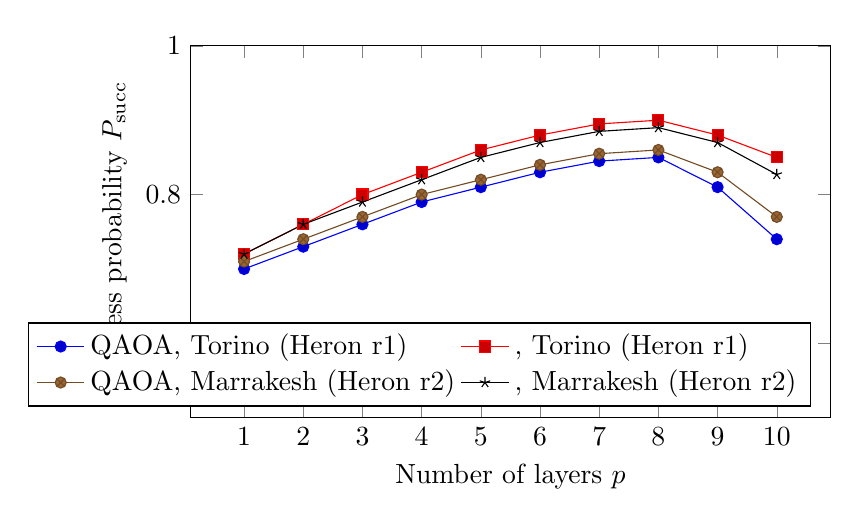
\begin{tikzpicture}
\begin{axis}[
  xlabel={Number of layers $p$}, ylabel={Success probability $P_{\mathrm{succ}}$},
  xtick={1,...,10}, ymin=0.5, ymax=1.0,
  legend pos=south east, legend cell align=left, legend columns=2,
  width=0.8\linewidth, height=0.52\linewidth]
  \addplot coordinates {(1,0.70) (2,0.73) (3,0.76) (4,0.79) (5,0.81) (6,0.83) (7,0.845) (8,0.85) (9,0.81) (10,0.74)};
  \addlegendentry{QAOA, Torino (Heron r1)}
  \addplot coordinates {(1,0.72) (2,0.76) (3,0.80) (4,0.83) (5,0.86) (6,0.88) (7,0.895) (8,0.90) (9,0.88) (10,0.85)};
  \addlegendentry{\deal, Torino (Heron r1)}
  \addplot coordinates {(1,0.71) (2,0.74) (3,0.77) (4,0.80) (5,0.82) (6,0.84) (7,0.855) (8,0.86) (9,0.83) (10,0.77)};
  \addlegendentry{QAOA, Marrakesh (Heron r2)}
  \addplot coordinates {(1,0.72) (2,0.76) (3,0.79) (4,0.82) (5,0.85) (6,0.87) (7,0.885) (8,0.89) (9,0.87) (10,0.827)};
  \addlegendentry{\deal, Marrakesh (Heron r2)}
\end{axis}
\end{tikzpicture}
\caption{Success probability versus number of layers for vanilla QAOA and \deal\ on IBM Torino (Heron r1) and IBM Marrakesh (Heron r2) for 20-qubit instances. Re-plotted from the values reported in \cite{guo2025deal} (rise from about 0.7 to a peak of 0.85--0.9 at seven to eight layers; \deal\ above QAOA throughout; \SI{14.81}{\percent} and \SI{7.40}{\percent} higher success at ten layers on Torino and Marrakesh); intermediate points are illustrative. The CZ gate count of the mapped circuit grows with $p$, and degradation sets in beyond roughly 41--43 CZ gates.}
\label{fig:nisq:deal-success}
\end{figure}

The energies confirm the picture. For all three problem families, \deal\ returned ground-state energies within a small margin of the classical optima in \cref{tab:nisq:problems}. That is, it returned near-optimal tours, packings and cuts on 20-qubit instances without a single optimiser iteration on the hardware \cite{guo2025deal}. Two further diagnostics were reported for a smaller 4-qubit instance with 16 basis states and 500 repetitions, on which the full output distribution could be examined.

The first diagnostic sorts the measured probabilities in decreasing order and accumulates them. The steepness of this cumulative-probability curve measures how concentrated the distribution is on its top states. The mean of the sorted probabilities was 0.1263 for \deal\ against 0.1149 for QAOA. The two performance-gap regions annotated between the mean curves in Fig.~3 of \cite{guo2025deal} have widths $\Delta=0.1065$ and $\Delta=0.0156$. Both results indicate that \deal\ places more of its probability mass on the leading, low-energy configurations.

The second diagnostic is the Kullback--Leibler divergence between the hardware distribution $\hat{P}$ and the noiseless reference $P$ from simulation,
\begin{equation}\label{eq:nisq:kl}
  D_{\mathrm{KL}}(P\,\Vert\,\hat{P}) = \sum_{\bm{x}} P(\bm{x})\log\frac{P(\bm{x})}{\hat{P}(\bm{x})},
\end{equation}
which decreased from about $10^{-1}$ at one layer to about $10^{-2}$ at the best depth for both methods. At the depths where success peaks, the hardware output is thus close to the ideal distribution. The advantage of \deal\ over QAOA comes from a better ideal distribution, that is, from the ansatz and the angles, rather than from a smaller hardware-induced distortion alone.

\section{QAWA: Quantum Approximate Walk Algorithm}\label{sec:nisq:qawa}

\deal\ removes the optimiser but keeps the QAOA structure: a problem-derived phase separator, an entangling mixer, and an output that is a sample from an entangled state. Its output is therefore still opaque. To confirm the quality of the solution, one must know the optimum in advance, as in the benchmarks above, or perform tomography of the output state, whose cost is exponential in $n$. The Quantum Approximate Walk Algorithm (\qawa) \cite{guo2025qawa} starts from the opposite end. It asks what a shallow circuit on a noisy device can learn about a problem whose instance is defined by \emph{classical data}. It designs the circuit so that every quantity it produces can be traced back to that data in closed form. \Cref{fig:nisq:qawa-pipeline} shows its three components and the flow of data between them.

% alt: Eight boxes in a loop: asset returns, copula targets, distributed walk learning, the multiplier oracle, mid-circuit records, classical preprocessing, the recovered copula and weights, and a classical check; a dashed arrow from preprocessing back to walk learning marks the angle update.
\begin{figure}[htbp]
\centering
\begin{tikzpicture}[
  font=\footnotesize,
  box/.style={draw,rounded corners=2pt,align=center,minimum height=9mm,inner sep=2pt,text width=28mm},
  data/.style={draw,fill=cbOrange!15,align=center,minimum height=9mm,inner sep=2pt,text width=28mm},
  arr/.style={-{Latex[length=2mm]},thick}]
  \node[data] (ret) at (0,0) {Asset returns};
  \node[box] (cop) at (3.8,0) {Copula targets};
  \node[box,fill=cbSky!20] (walk) at (7.6,0) {Distributed walk learning};
  \node[box,fill=cbGreen!15] (orc) at (11.4,0) {Multiplier oracle};
  \node[box] (rec) at (11.4,-2.4) {Mid-circuit records};
  \node[box] (pre) at (7.6,-2.4) {Classical preprocessing};
  \node[data] (out) at (3.8,-2.4) {Copula and weights};
  \node[box,fill=cbPurple!15] (ver) at (0,-2.4) {Classical check};
  \draw[arr] (ret) -- (cop);
  \draw[arr] (cop) -- (walk);
  \draw[arr] (walk) -- (orc);
  \draw[arr] (orc) -- (rec);
  \draw[arr] (rec) -- (pre);
  \draw[arr] (pre) -- (out);
  \draw[arr] (out) -- (ver);
  \draw[arr,dashed] (pre.north) -- node[right,font=\scriptsize]{update $\theta$} (walk.south);
\end{tikzpicture}
\caption{The \qawa\ pipeline. Classical data enter through the multiplier oracle (\cref{sec:nisq:oracle}), walk learning (\cref{sec:nisq:walk}) updates its angles from the measured statistics, and classical preprocessing (\cref{sec:nisq:interp}) returns the copula and the portfolio weights, which are checked classically.}
\label{fig:nisq:qawa-pipeline}
\end{figure}

\subsection{Classical-Data-Traceable Oracle}\label{sec:nisq:oracle}

The core component is an oracle that loads classical data into a quantum register in a way that is both shallow and traceable. We call its circuit the multiplier oracle (\cref{fig:nisq:qawa-oracle}). The register is split into an \emph{address} part $A$ of $n_{a}$ qubits and a \emph{data} part $B$ of $n_{b}$ qubits. A layer of Hadamard gates puts $A$ into the uniform superposition over the $2^{n_{a}}$ addresses. Each address qubit $a$ then controls an $R_{Y}(\theta_{ab})$ rotation on each data qubit $b$. The angle $\theta_{ab}$ encodes one classical datum, for instance the return of asset $b$ in scenario $a$, through the amplitude-encoding map $\theta=2\arcsin\sqrt{v}$ of \cref{sec:bg:encoding}.

Rotations about the same axis add. Conditioned on the address string $\bm{a}=(a_{1},\dots,a_{n_{a}})$, data qubit $b$ therefore receives the total rotation $\Theta_{b}(\bm{a})=\sum_{j}a_{j}\theta_{jb}$, and the joint state after the ladder is
\begin{equation}\label{eq:nisq:oracle-state}
  \ket{\Phi} = \frac{1}{\sqrt{2^{n_{a}}}}\sum_{\bm{a}\in\{0,1\}^{n_{a}}} \ket{\bm{a}}_{A}\otimes\bigotimes_{b=1}^{n_{b}}
  \Bigl[\cos\tfrac{\Theta_{b}(\bm{a})}{2}\ket{0}+\sin\tfrac{\Theta_{b}(\bm{a})}{2}\ket{1}\Bigr]_{B}.
\end{equation}
A final layer of $R_{Z}(\pi/2)$ rotations on $B$ fixes the phase reference of the data register. It commutes with the $Z$-basis readout of $B$, so it does not change the marginal statistics reported below. But it matters when the oracle is composed with subsequent walk steps that act on the same register. All qubits are then read out in the $Z$ basis.

% alt: Quantum circuit of the QAWA multiplier oracle with two address qubits and two data qubits. Hadamard gates on the address qubits are followed by a ladder of controlled-RY rotations, each address qubit controlling a rotation with a data-dependent angle on each data qubit. The data qubits receive RZ(pi/2) rotations and all four qubits are measured in the Z basis.
\begin{figure}[htbp]
\centering
\begin{quantikz}[row sep={0.75cm,between origins},column sep=0.3cm,font=\small]
\lstick[2]{address $A$} & \gate{H} & \ctrl{2} & & \ctrl{3} & & & \meter{Z} \\
 & \gate{H} & & \ctrl{1} & & \ctrl{2} & & \meter{Z} \\
\lstick[2]{data $B$} & & \gate{R_Y(\theta_{11})} & \gate{R_Y(\theta_{21})} & & & \gate{R_Z(\pi/2)} & \meter{Z} \\
 & & & & \gate{R_Y(\theta_{12})} & \gate{R_Y(\theta_{22})} & \gate{R_Z(\pi/2)} & \meter{Z}
\end{quantikz}
\caption{The \qawa\ multiplier oracle for $n_{a}=2$ address and $n_{b}=2$ data qubits. Hadamard gates prepare the address superposition; each address qubit controls an $R_{Y}(\theta_{ab})$ rotation encoding one classical datum on each data qubit; an $R_{Z}(\pi/2)$ layer fixes the phase of the data register before $Z$-basis readout. Every measured probability is a closed-form trigonometric function of the angles $\theta_{ab}$ (\cref{eq:nisq:oracle-state}). Schematic of the oracle in \cite{guo2025qawa}.}
\label{fig:nisq:qawa-oracle}
\end{figure}

Three properties follow from \cref{eq:nisq:oracle-state}. First, the oracle is \emph{traceable}. The probability of observing data bit $b=1$ together with address $\bm{a}$ is $2^{-n_{a}}\sin^{2}(\Theta_{b}(\bm{a})/2)$, an explicit function of the classical inputs. The pairwise statistic $\expval{Z_{b}Z_{b'}}$ averaged over addresses is $2^{-n_{a}}\sum_{\bm{a}}\cos\Theta_{b}(\bm{a})\cos\Theta_{b'}(\bm{a})$, a \emph{product} of two data-dependent quantities averaged over scenarios. This is why we call the circuit a multiplier: it computes, in superposition over all scenarios, exactly the products whose averages define correlations. Any output can therefore be checked classically in time polynomial in $n_{a}$ and $n_{b}$ for a given set of addresses. The whole output distribution can be checked in time $\bigO{2^{n_{a}}n_{b}}$, which is polynomial when the address register is small.

Second, the oracle is \emph{shallow}. Each controlled rotation compiles to two CNOT gates, and the rotations on different data qubits controlled by the same address qubit can be scheduled in parallel. The ladder over $n_{b}$ data qubits therefore has CNOT depth $\bigO{n}$ in the total qubit count. This contrasts with the $\bigO{n^{2}}$ two-qubit gates of a dense QAOA cost layer. It also contrasts with the $\bigO{n^{2}}$ measurement settings, each with its own circuit, that pairwise tomography would need to extract the same correlations from a generic state \cite{huang2020shadows}.

Third, the oracle is a special case of the uniformly controlled rotations \cite{mottonen2004ucr} on which the \qcrank\ encoding of \cref{sec:bg:encoding} is built \cite{balewski2024qcrank}. \qcrank\ loads one datum per address into a data qubit by a full uniformly controlled rotation. The multiplier oracle uses only the linear, single-control terms of that rotation, and it trades exactness of the loaded values for a depth linear rather than exponential in $n_{a}$. This approximation gives the algorithm its name.

\subsection{Distributed Approximate Walk Learning}\label{sec:nisq:walk}

The oracle alone loads data. The walk uses it to learn. In a discrete-time quantum walk \cite{childs2009quantumwalk}, a coin operation on an internal register is followed by a shift conditioned on the coin. The walker's position distribution after $t$ steps depends on the coin angles. \qawa\ uses the multiplier oracle as a data-dependent coin: the data register $B$ acts as the walker, the address register $A$ as the coin, and the controlled-rotation ladder as the coin-conditioned shift. One application of the oracle is thus one approximate walk step, and the angles $\theta_{ab}$ are the walk's parameters.

The learning task is to choose the angles so that the distribution of the data register matches a target distribution $P_{\mathrm{target}}$ derived from the problem. The loss is the Kullback--Leibler divergence $D_{\mathrm{KL}}(P_{\mathrm{target}}\Vert\hat{P}_{\theta})$ of \cref{eq:nisq:kl} between the target and the measured distribution. For the portfolio application, the target is a \emph{copula}. By Sklar's theorem \cite{sklar1959copula}, the joint distribution of the returns of several assets factorises into its marginals and a copula that carries the dependence structure alone. The copula is what a portfolio optimiser needs, because the marginals are known and the risk comes from the dependence. \qawa\ transforms the historical returns of each asset to uniform marginals. It discretises the pairwise copula of each pair of assets on a grid indexed by the address register and learns one set of oracle angles per pair.

The learning is \emph{distributed}. Independent sub-walks learn the $\binom{n_{b}}{2}$ pairwise copulas, on separate GPU ranks in simulation or in separate hardware jobs. The learned angles are then reassembled into a single oracle whose pairwise statistics $\expval{Z_{b}Z_{b'}}$ reproduce all pairwise dependencies at once. After each iteration, the classical controller updates the angles from the measured statistics by plain gradient descent with a fixed learning rate $\eta$ on the KL loss. Because each measured statistic has the closed form of \cref{sec:nisq:oracle}, the update can be computed and verified classically. In the experiments below, the divergence fell below $0.01$ after about 75 of the 150 training iterations (the fitted decay is $\mathrm{KL}(t)=0.082\,e^{-0.031t}+0.004$ \cite{guo2025qawa}). This is one to two orders of magnitude below the evaluation count of a black-box QAOA optimiser.

\subsection{Interpretability Through Mid-Circuit Measurement Preprocessing}\label{sec:nisq:interp}

The final component of \qawa\ is a reading of QAOA-style outputs that does not require tomography. In a generic variational circuit, the only accessible information is the final bit-string distribution, and relating it to the problem requires reconstruction of the state. \qawa\ instead records mid-circuit measurement data, the outcomes of the address register together with the data register, and processes them classically. The address outcome identifies the scenario, and the data outcome is a closed-form function of that scenario's data, so the pair can be interpreted directly. The empirical conditional frequencies $\hat{P}(b\mid\bm{a})$ estimate $\sin^{2}(\Theta_{b}(\bm{a})/2)$, and the empirical pairwise statistics estimate the products defined in \cref{sec:nisq:oracle}.

Recovery of all $\binom{n}{2}$ pairwise correlations of $n$ data qubits from these records needs $\bigO{n^{2}}$ estimated quantities. Each comes from the same measurement data rather than from separate tomographic circuits, and the estimates can be checked against the classical data that generated the angles. Solution quality is therefore verifiable in polynomial time. Given the returned portfolio weights, the expected return and risk can be computed from the recovered copula and compared with the classical baseline, without trust in the quantum device. A classical party who did not run the quantum computation can thus audit the output. This property anticipates the verification theme of \cref{ch:qec}.

\section{QAWA Experimental Setup and Results}\label{sec:nisq:qawa-results}

The application reported in \cite{guo2025qawa} is a four-asset portfolio drawn from the S\&P~500, made up of Apple (AAPL), Microsoft (MSFT), Johnson~\&~Johnson (JNJ) and Exxon Mobil (XOM). These assets were chosen to span technology, health care and energy, so that the pairwise dependencies are genuinely different. The historical returns were transformed to uniform marginals, and the six pairwise copulas were the learning targets. Simulations used \qiskit\ 2.2 with the Aer state-vector back end on the TTU HPCC and NERSC systems. They were extended to 20 qubits to establish the scaling of the oracle's depth and of the learning dynamics. The shallow oracle circuits up to the measurement layer were also cross-checked with the \qgear\ pipeline of \cref{ch:qgear}.

Hardware runs used IBM Pittsburgh, a 156-qubit Heron~r3 processor (\cref{tab:nisq:hw}), with 8,192 shots per circuit and 20 independent runs per configuration. Averages and noise floors could thus be estimated. The baseline portfolio was the classical mean--variance allocation computed from the empirical covariance. The noise floor was estimated from the spread of the hardware results across the 20 runs.

\Cref{fig:nisq:qawa-kl} shows the learning dynamics. From an uninformative initialisation, the KL divergence between the target copula and the measured distribution decreased monotonically and reached 0.01 after about 75 iterations. At that point, all six pairwise correlation coefficients of the four assets had been recovered from the pairwise statistics of the oracle \cite{guo2025qawa}. The curve flattens below $10^{-2}$, the level set by the shot noise of the finite sample per iteration rather than by the expressivity of the oracle.

On IBM Pittsburgh, the portfolio constructed from the hardware-recovered copula achieved an average improvement of \SI{5.4}{\percent} over the baseline portfolio across the 20 runs. It also achieved an advantage of \SI{8.1}{\percent} above the noise floor, as reported in \cite{guo2025qawa}. A QAOA formulation of the same portfolio QUBO, run under the same shot budget, did not match this result even with additional optimiser iterations. \qawa\ needed none beyond its walk-learning schedule. Every quantity that enters the portfolio construction is a closed-form function of the measured statistics. The entire chain from hardware counts to portfolio weights was therefore re-verified classically in polynomial time.

% alt: Log-scale line chart of Kullback-Leibler divergence versus learning iteration from 0 to 100 for the four-asset copula learning task. The curve decreases from about 0.5 at iteration 0 to 0.01 at about iteration 75 and then flattens; a dashed horizontal line marks the 0.01 convergence level.
\begin{figure}[htbp]
\centering
\begin{tikzpicture}
\begin{axis}[
  ymode=log, xlabel={Walk-learning iteration}, ylabel={$D_{\mathrm{KL}}(P_{\mathrm{target}}\,\Vert\,\hat{P}_{\theta})$},
  xmin=0, xmax=100, ymin=0.005, ymax=1,
  legend pos=north east, legend cell align=left,
  width=0.75\linewidth, height=0.5\linewidth]
  \addplot coordinates {(0,0.52) (5,0.35) (10,0.24) (15,0.17) (20,0.12) (30,0.07) (40,0.045) (50,0.028) (60,0.018) (70,0.012) (75,0.010) (85,0.0095) (100,0.009)};
  \addlegendentry{four-asset copula (mean over six pairs)}
  \addplot[cbGray,dashed,no marks] coordinates {(0,0.01) (100,0.01)};
  \addlegendentry{convergence level 0.01}
\end{axis}
\end{tikzpicture}
\caption{Kullback--Leibler divergence between the target copula and the distribution produced by the \qawa\ oracle versus walk-learning iteration for the four-asset S\&P~500 portfolio. Re-plotted from the values reported in \cite{guo2025qawa} (convergence to 0.01 in about 75 iterations; all six pairwise correlations recovered); intermediate points are illustrative.}
\label{fig:nisq:qawa-kl}
\end{figure}

\Cref{tab:nisq:compare} summarises how vanilla QAOA, \deal\ and \qawa\ differ along the dimensions that RQ3 asks about:
\begin{itemize}
\item the source of the circuit structure;
\item the number of circuit evaluations on the classical side;
\item the circuit depth;
\item the mitigation and interpretation of the output;
\item the cost of verification.
\end{itemize}
The progression from column to column is the progression of the chapter: from search over an unstructured parameter space, to structure imported from the problem and the device, to structure imported from the data with a verifiable output.

\begin{table}[htbp]
\caption{Comparison of vanilla QAOA, \deal\ and \qawa\ along the dimensions addressed by RQ3. $p$ is the number of layers, $|E|$ the number of non-zero QUBO couplings, $n$ the number of qubits. Compiled from \cite{farhi2014qaoa,guo2025deal,guo2025qawa}.}
\label{tab:nisq:compare}
\centering\small
\begin{tabular}{@{}>{\raggedright\arraybackslash}p{0.2\linewidth}>{\raggedright\arraybackslash}p{0.24\linewidth}>{\raggedright\arraybackslash}p{0.24\linewidth}>{\raggedright\arraybackslash}p{0.24\linewidth}@{}}
\toprule
Property & Vanilla QAOA & \deal & \qawa \\
\midrule
Source of structure & problem Hamiltonian only & problem (QPN weights) and device (calibration, topology) & classical data (walk angles, copula targets) \\
Parameter initialisation & random or generic ramp & closed form from $Q$ (\cref{eq:nisq:init}) & data-encoding angles, refined by walk learning \\
Classical outer loop & black-box optimiser, $10^{2}$--$10^{3}$ noisy evaluations & none (direct angles); Bayesian choice of $p$ & distributed walk learning, about 75 iterations \\
Two-qubit gate depth & $\bigO{p\,|E|}$ plus SWAPs & $\bigO{p\,|E|}$, heavy edges on adjacent low-error couplers & $\bigO{n}$ CNOT depth per oracle \\
Error mitigation & none & adaptive digital ZNE with delay/identity insertion, $\lambda\in\{1,2\}$ & classical preprocessing of mid-circuit data; noise floor from repeated runs \\
Interpretability & bit-string energies only & QNRE separates noise-limited from parameter-limited error & every output a closed-form function of the input data \\
Verification & know the optimum, or tomography $\bigO{4^{n}}$ & energy re-evaluation against known optimum & polynomial time; $\bigO{n^{2}}$ estimated pairwise statistics \\
Hardware demonstration & (baseline runs) & IBM Torino, IBM Marrakesh, 20 qubits, 10 layers & IBM Pittsburgh, four assets; simulation to 20 qubits \\
\bottomrule
\end{tabular}
\end{table}

\section{Discussion and Limitations}\label{sec:nisq:discussion}

The results of this chapter support the claim of RQ3 that structure beats search on today's devices. But they also delimit the claim, and we record the limits here. The first limit concerns \emph{scale}. All hardware results are for 20 qubits or fewer and for at most ten layers. The falling branches in \cref{fig:nisq:deal-success} show this limit. At 41--43 CZ gates, the devices used here are already near the depth at which output distributions lose their structure. \deal\ pushes the useful depth by two layers and the success rate by up to fifteen per cent. This is significant for practice but does not change the exponent: larger instances need more couplings, and more couplings need more CZ gates. No initialisation or mapping heuristic can substitute for lower gate errors.

The closed-form angles of \cref{eq:nisq:init} were tuned on the three problem families in \cref{tab:nisq:problems}. The scale factors $\lambda_{\gamma},\lambda_{\beta}$ may need adjustment for QUBOs with very different coefficient distributions. Whether a universal setting exists is an open question that the Bayesian machinery of \cref{sec:nisq:zne} could be extended to answer.

The second limit concerns \emph{what the mapping can fix}. The greedy solution of \cref{eq:nisq:mapping} places the heaviest edges well. But on a heavy-hexagonal graph of degree three, a dense 20-variable QUBO with 190 couplings cannot avoid SWAP chains for most of its edges. The mapping determines which edges pay the SWAP cost, not whether the cost is paid. Devices with higher connectivity, or the circuit-cutting approach of \cref{ch:qml} that removes the worst edges altogether, address the remaining cost from different directions.

The third limit concerns \emph{approximation in \qawa}. The multiplier oracle is exact for the single-control terms of a uniformly controlled rotation and drops the higher-order terms. Copulas with strong tail dependence have densities far from products of pairwise factors. For them, the approximate walk may converge to a KL divergence floor above the shot-noise level. The four-asset experiment does not probe this regime. The 20-qubit simulations only establish that the depth and the learning dynamics scale, not that the approximation stays accurate for arbitrary targets. The full \qcrank\ encoding is the natural fallback: its depth is exponential in the address register, but it is exact. The trade-off between the two is exactly the encoding question of \cref{ch:qml}.

The fourth limit concerns the \emph{baselines}. Vanilla QAOA with a linear-ramp start and a generic optimiser is the standard comparison in the literature. But stronger classical heuristics exist for each of the problems considered, and no claim of quantum advantage over them is made here or in the underlying papers. The contribution is methodological. On a fixed noisy device with a fixed budget, structure-aware circuits reach higher success with fewer evaluations, and they produce outputs whose quality can be judged.

\section{Relation to the Other Chapters}\label{sec:nisq:relation}

The two methods of this chapter obtain structure from complementary sources. The contrast, summarised in \cref{fig:nisq:structure-sources}, is instructive for the dissertation as a whole. \deal\ derives structure \emph{from the problem}: the QUBO coefficients fix the angles through \cref{eq:nisq:init} and the placement through \cref{eq:nisq:mapping}. The hardware enters only through calibration data that modulate that placement and the noise-scaling schedule. Its circuits remain QAOA-like, and its outputs remain samples judged by their energy.

\qawa\ derives structure \emph{from the data}: the instance is a set of numbers, the oracle loads them by amplitude encoding, and the walk learns from their statistics. The problem enters only through the choice of target distribution. Its circuits are data loaders rather than phase separators, and its outputs are statistics whose meaning is fixed by construction. The two are ends of a spectrum, not competitors. Their hinge is the amplitude-encoding angle $2\arcsin\sqrt{w}$, the initialisation of \deal\ and the oracle angle of \qawa. In both cases, the numbers that define the instance become rotation angles without an optimiser in between.

% alt: Two rows of boxes. Top row, DEAL: QUBO matrix, QPN weights, angle map, QAOA-like circuit, samples, with a calibration-data box feeding the circuit. Bottom row, QAWA: classical data, angle map, data-loading oracle, statistics, with a target-distribution box feeding the oracle. A dashed line links the two angle maps with the note that no optimiser sits between the numbers and the angles.
\begin{figure}[htbp]
\centering
\begin{tikzpicture}[
  font=\footnotesize,
  box/.style={draw,rounded corners=2pt,align=center,minimum height=9mm,inner sep=2pt,text width=24mm},
  data/.style={box,fill=cbOrange!15},
  ang/.style={box,fill=cbSky!20},
  cir/.style={box,fill=cbGreen!15},
  arr/.style={-{Latex[length=2mm]},thick}]
  \node[font=\footnotesize\bfseries,anchor=west] at (-1.3,1.0) {DEAL: structure from the problem};
  \node[data] (q)  at (0,0) {QUBO matrix $Q$};
  \node[box]  (w)  at (3.1,0) {QPN weights};
  \node[ang]  (a1) at (6.2,0) {angle $2\arcsin\sqrt{w_i}$};
  \node[cir]  (c1) at (9.3,0) {QAOA-like circuit};
  \node[data] (o1) at (12.4,0) {Samples};
  \node[data] (cal) at (9.3,-1.5) {Calibration data};
  \draw[arr] (q)--(w); \draw[arr] (w)--(a1); \draw[arr] (a1)--(c1); \draw[arr] (c1)--(o1); \draw[arr] (cal)--(c1);
  \node[font=\footnotesize\bfseries,anchor=west] at (-1.3,-2.6) {QAWA: structure from the data};
  \node[data] (d)  at (0,-3.6) {Classical data};
  \node[ang]  (a2) at (6.2,-3.6) {angle $2\arcsin\sqrt{v_{ab}}$};
  \node[cir]  (c2) at (9.3,-3.6) {Data-loading oracle};
  \node[data] (o2) at (12.4,-3.6) {Statistics};
  \node[data] (tgt) at (9.3,-5.1) {Target distribution};
  \draw[arr] (d)--(a2); \draw[arr] (a2)--(c2); \draw[arr] (c2)--(o2); \draw[arr] (tgt)--(c2);
  \draw[dashed,cbGray] (a1.south) -- node[right,font=\scriptsize,align=left,text=cbGray]{same map,\\ no optimiser} (a2.north);
\end{tikzpicture}
\caption{Two sources of structure. \deal\ turns QUBO coefficients into rotation angles; \qawa\ turns classical data into rotation angles. The same amplitude-encoding angle appears in both, with no optimiser between the numbers and the angles.}
\label{fig:nisq:structure-sources}
\end{figure}

Both methods depend on the simulation substrate of \cref{ch:qgear}. The 20-qubit, 10-layer \deal\ circuits were simulated noiselessly through \qgear\ on A100 GPUs before every hardware submission. This confirmed that the directly initialised angles produce low-energy states, and it provided the reference distributions $P$ in \cref{eq:nisq:kl}. Without GPU acceleration, a trace of ten layer counts across three problem families and two devices would have consumed days of CPU time per iteration of the design. The \qawa\ oracles were simulated up to 20 qubits with the same pipeline, up to their measurement layer. The mid-circuit measurement path is one of the gate-set limitations noted in \cref{sec:qgear:discussion}.

In retrospect, \qawa's data-traceable oracle is another instance of the theme that \cref{ch:qml} developed fully: the interface between classical data and the quantum register should be a structured, vectorised encoding whose outputs can be read without tomography. The \qcrank\ encoding and its \shardq\ cutting, the vectorised dot products of the \vqt\ transformer, and the exact quantum arithmetic of \nnqa\ all generalise the multiplier oracle in different directions. They trade depth for exactness or for learnability. The hardware-aware mapping of \deal\ likewise has its counterpart in \shardq. There, the entanglement distance of the encoder decides where to cut a circuit, and the calibrated coupling map decides where its sub-circuits run. The polynomial-time verifiability of \qawa's output, together with the QNRE metric's separation of noise-limited from parameter-limited error, foreshadows the auditing questions of \cref{ch:qec}. Once quantum computations run on shared cloud hardware whose noise a user cannot control, a classical check of an output is not a convenience but a requirement.

\section{Summary}\label{sec:nisq:summary}

This chapter presented two hardware-aware approaches to combinatorial optimisation on noisy superconducting processors. \deal, summarised in \cref{alg:deal}, combines four elements:
\begin{itemize}
\item a closed-form initialisation derived from the QUBO coefficients through Qubit Prioritization Normalization, which replaces the black-box parameter search of QAOA;
\item a dynamic mapping of logical qubits to the device that weighs interaction strength against calibrated error;
\item $R_{XX+YY}$ mixer blocks compiled to native maximally entangling gates;
\item an adaptive digital zero-noise extrapolation for the residual noise.
\end{itemize}
On IBM Torino and IBM Marrakesh, 20-qubit, 10-layer \deal\ circuits achieved success rates \SI{14.81}{\percent} and \SI{7.40}{\percent} higher than vanilla QAOA at ten layers. They matched with seven layers what QAOA needed nine for, and they returned near-optimal energies for TSP, knapsack and MaxCut instances, as reported in \cite{guo2025deal}.

\qawa\ introduces a classical-data-traceable oracle of linear CNOT depth and learns copulas by a distributed approximate quantum walk. It makes the outputs interpretable and verifiable in polynomial time through classical preprocessing of mid-circuit measurement data. On IBM Pittsburgh, it recovered all six pairwise correlations of a four-asset S\&P~500 portfolio and converged to a KL divergence of 0.01 in about 75 iterations. It improved on the baseline portfolio by \SI{5.4}{\percent} on average, \SI{8.1}{\percent} above the noise floor, as reported in \cite{guo2025qawa}.

Both methods were pre-validated with the \qgear\ pipeline of \cref{ch:qgear}. Together they answer RQ3 in the affirmative for the scales accessible today, and they close the loop with the question that preceded it. The data-derived structure that makes these shallow circuits interpretable is the same structured, vectorized data interface that \cref{ch:qml} built for learning (RQ2). The next chapter asks what circuits of either kind will cost once they must respect fault-tolerant budgets.
